%% Template for Master thesis
%% ===========================
%%
%% You need at least KomaScript v3.0.0,
%% e.g. available in Texlive 2009
\documentclass  [
  paper    = a4,
  BCOR     = 10mm,
  twoside,
  fontsize = 12pt,
  fleqn,
  toc      = bibnumbered,
  toc      = listofnumbered,
  numbers  = noendperiod,
  headings = normal,
  listof   = leveldown,
  version  = 3.03
]                                       {scrreprt}

% used pagages
\usepackage     [utf8]          {inputenc}
\usepackage     [T1]            {fontenc}
\usepackage                     {color}
\usepackage                     {amsmath}
\usepackage                     {graphicx}
\usepackage     [english]       {babel}
\usepackage                     {natbib}
\usepackage                     {hyperref}
\usepackage						{cleveref}
\usepackage						{subfigure}
% links
\definecolor{darkblue}{rgb}{0.0,0.0,0.4}
\definecolor{darkgreen}{rgb}{0.0,0.4,0.0}
\hypersetup{
    colorlinks,
    linkcolor=black,
    citecolor=darkgreen,
    urlcolor=darkblue
}
%\renewcommand{\partname}{}
%\renewcommand{\thepart}{}

\begin{document}
  %% title pages similar to providet template instead of maketitle
  %% this will generate title pages similar to the template provided
%% by the Department of Physics and Astronomy Heidelberg
%%
%% More information:
%% http://www.physik.uni-heidelberg.de/aktuelles/studium/
%% (PDF link: ...studium/download/145/Vorlage_Diplomarbeit_Formular.pdf)

%% Titleintro
\thispagestyle{empty}
\begin{center}
  \renewcommand{\baselinestretch}{2.00}
  \Large\sffamily
  Department of Physics and Astronomy\\
  \large University of Heidelberg
  \par\vfill\normalfont
  Master thesis\\
  in Physics\\
  submitted by\\
  Elsa  Wilken\\
  born in Hamburg\\
  2018
\end{center}
\newpage

%% Titlepage
\thispagestyle{empty}
\begin{center}
  \renewcommand{\baselinestretch}{2.00}
  \Large\bfseries\sffamily
    Retrieval Advances of BrO/\ce{SO2}              \\
    Molar Ratios from NOVAC\\
  \par
  \vfill
  \large\normalfont
  This Master thesis has been carried out by Elsa Wilken\\
  at the\\
  Institute for Environmental Physics, University of Heidelberg, Germany\\
  under the supervision of\\
  Prof. Ulrich Platt,\\
  Dr. Nicole Bobrowski,\\
  Florian Dinger
  %% additionally insert second supervisor here if carrying out an
  %% external diploma thesis. Reduce vspace in L. 44 accordingly.
\end{center}\par
\vspace{5\baselineskip}

% reset baselinestretch
\renewcommand{\baselinestretch}{1.00}\normalsize % or english title page
  %% Abstract page
%% =============
%%
%% Content of abstract pages has been put into seperate pages to simplify
%% word counting. Use e.g. the unix command
%%   wc abstract-ger.tex
%% or
%%   wc abstract-eng.tex
%% to get the number of words contained in these files.
\thispagestyle{empty}
\begin{center}
  \begin{minipage}[c][0.48\textheight][b]{0.9\textwidth}
    \small
    \textbf{Optimierte Bestimmung des molaren BrO/\ce{SO2} Verhältnisses aus NOVAC Daten
    }\par
    \vspace{\baselineskip}
    %% Latex markup und Zitate funktionieren auch hier


Die Messung der absoluten Menge und von Konzentrationsverhältnissen vulkanischer Gas Emissionen geben Einsicht in magmatische Prozesse. Das Network for Observation of Volcanic and Atmospheric Change (NOVAC) besteht aus einem System von automatisierten UV-Spektrometern, welche die Gas Emissionen der Vulkane aufzeichnen. Die Emission von BrO und \ce{SO2} kann mithilfe von Differenzieller optischer Absorptionsspektroskopie (DOAS) aus den aufgenommen Spekren bestimmt werden wobei die optische Absorption in der Fahne mit einem Reference Spectrum verglichen wird. Dies setzt voraus, dass das Reference Spectrum frei von Vulkanische Gasen ist. Typischerweise wird das Reference Spectrum für einen Scan bei einem Elevationswinkel aufgenommen welcher welcher so gewählt wird dass das Instrument nicht in die Fahne schaut. Es hat sich jedoch gezeigt, dass auch diese Spektren noch durch Vulkanische Emissionen verunreinigt sein können. Als alternative Referenzspektren könnten 1) ein theoretisches Solar Atlas Spektrum oder 2) ein nicht verunreinigtes Referenz Spektrum des selben Messgeräts dienen. Option 1) hat den Nachteil einer verringerten Messgenauigkeit, da Instrumenteneffekte hier modelliert werden müssen und ist daher nur für das typischerweise in hoher Konzentration vorkommende \ce{SO2} anwendbar. Option 2) setzt voraus, dass das Referenzspektrum unter ähnlichen Wetter- und Strahlungsbedingungen aufgenommen wurde. Wir verwenden die erste Methode um (\ce{SO2}) Kontaminierung zu identifizieren und greifen für die Bestimmung der Gas Konzentration auf die zweite Methode zurück um eine hohe Qualität der Messung sicher zu stellen. Im Folgenden stellen wir unsere Methode für NOVAC Daten von den Vulkanen Tungurahua und Nevado Del Ruiz vor.
  \end{minipage}\par
  \vfill
  \begin{minipage}[c][0.48\textheight][b]{0.9\textwidth}
    \small
    \textbf{Retrieval advances of BrO/\ce{SO2} molar ratios from NOVAC
    }\par
    \vspace{\baselineskip}
    %% Latex markup and citations may be used here

%Measurements of magnitude and composition of volcanic gas emissions allow insights in magmatic processes. Within the Network for Observation of Volcanic and Atmospheric Change(NOVAC) automatically scanning UV-spectrometers are monitoring gas emission at volcanoes. The emissions of BrO and \ce{SO2} can be retrieved from the recorded spectra by applying Differential Optical Absorption Spectroscopy(DOAS) and comparing the optical absorption of the volcanic plume to the background. Therefore, the background spectrum must not be affected by volcanic influence. Conventionally, the background spectrum is taken from the same scan but from an elevation angle which has been identified to be outside of the volcanic plume. However, experience shows those background spectra can still be contaminated by volcanic gases.  Alternatively, background spectra can be derived from 1) a theoretical solar atlas spectrum or 2) a volcanic-gas-free background spectrum recorded by the same instrument at another time. 1) comes with a drawback of reduced precision, as the instrumental effects have to be modeled and added to the retrieval. For 2), the alternative background spectrum should be recorded at similar conditions with respect to meteorology and radiation. We use the first option to check for contamination and the second to evaluate the spectra to maintain a good fit quality. We present our approach and its results when applied on NOVAC data from Tungurahua and Nevado del Ruiz.

Measurements of magnitude and composition of volcanic gas emissions allow insights into magmatic processes. In this thesis, the concentration ratio of BrO and \ce{SO2} is analyzed. The measurements are performed with scanning UV-spectrometers provided by the "Network for Observation of Volcanic and Atmospheric Change (NOVAC)".
The concentrations are then retrieved by applying Differential Optical Absorption Spectroscopy (DOAS).
For this purpose, especially weak absorbers like BrO require a gas-free reference spectrum to eliminate the Fraunhofer structures.
However, with the conventional evaluation approach, it is still possible that the chosen same-time-reference spectra are contaminated. Alternative reference spectra could be (1) a theoretical solar atlas spectrum or (2) a temporal shifted uncontaminated reference spectrum which is recorded by the same instrument. (1) comes with the drawback of a decreased measurement precision, as instrumental effects must be modeled, while (2) only works with a reference that is recorded under similar conditions as the measurement spectrum. In this work, a new approach is presented which uses (1) for the identification of (\ce{SO2}) contamination and (2) for the actual measurement of the gas concentration. The novel approach sidesteps the systematic underestimation of the concentration and increases the amount of reliable data by approximately 30\%. Moreover, we are able to prove the occurrence of BrO contamination.
  \end{minipage}
\end{center}


  \tableofcontents
  %% Put your contents here
	\chapter{Introduction}	
	
%% Introduction page
%% =============
%%
Volcanic activities on Earth have  always shaped the earth surface and influenced atmospheric processes. Volcanoes are often particularly recognized by their dramatic consequences of a major volcanic eruption. But volcanoes influence our lives in more than this way. Volcanic gases can effect the weather (timescales of days to weeks) or the climate (timescales of months to years) \cite{schmidt2015volcanismarticle}.
Examples are the lake eruption in Iceland (1783-1784) followed by a very hot summer and a cold winter in central Europa \cite{thordarson2003atmospheric} and the Tambora eruption, indonesia in 1815 which caused the "year without summer" in 1816.\\
%
\newline
%
Considering the plate tectonics of earth  most volcanoes are caused by diverging or converging of the continental plates and therefore located at the margins of the continental plates.
Another possibility for occurrence of volcanoes is the the interior of continental or oceanic shelves. \cite{schmincke2000vulkanismus}\\
The most abundant volatile species released during a volcanic eruption are water vapour (H$_2$O; relative amount of the plume: 50\%-90\%) and carbon dioxide (CO$_2$; relative amount of the plume: 1\%-40\%) \cite{platt2015quantification}. But the short effects of those two gases are rather low since there effect on atmospheric composition is negligibly due to the high abundance of atmospheric H$_2$O and CO$_2$. But on timescales of the age of the earth the volcanic emission of H$_2$O and CO$_2$ are the source of our current atmosphere. \cite{schmidt2015volcanism}\\ 
A typically volcanic plume consists of many different gases alongside H$_2$O and CO$_2$  sulfur dioxide (SO$_2$) contributes with 1\%-25\% to the plume, hydrogen sulfide (H$_2$S) with 1\%-10\% and hydrogen chloride with (HCl) 1\%-10\%. Furthermore there are trace gases for example carbon disulfide (CS$_2$), carbon sulfide (COS) carbon monoxide (CO) hydrogen fluoride (HF) and hydrogen bromide (HBr) \cite{platt2015quantification}\\
%
A decrease of stratospheric ozone (O$_3$) has been observed after the eruption of  El Chickon in 1982 and the eruption of mount Pinatubo 1991. A depletion stratospheric O$_3$ results in ozone holes. The depletion comes from volcanic aerosols which serve anthropogenic chlorine/bromine into more reactive forms \cite{solomon1998ozone}. 
%
Volcanic gases can alter the radiative balance of the earth in timescales relevant for climate change due to scatter and absorption of solar radiation \cite{schmidt2015volcanism}.\\
%
The gas composition of the volcano plume change with activity and could be a indication for the processes inside the earth.\\ 
%
In this work we are particularly interested in the ratio of BrO and SO$_2$. The halogen sulfur ratio is a proxy for volcanic processes. Therefore we make the assumption
that the ratio of BrO and SO2 contains informations about its degassing source depth. A change in BrO/SO2 prior to eruption was observed at Etna and Nevado del Ruiz.\\
%
\newline
%
To gain further knowledge about the volcanoes the Network for Observation of Volcanic and Atmospheric Change (NOVAC) was installed. NOVAC is a Network of DOAS Instruments located next to about 30 volcanoes in America, Africa and Europe. At every Volcano there are two to four DOAS Instruments installed, recording record back-scattered solar radiation spectra at different viewing angles.\\
NOVAC is a network which produces a large amount of data and we have the chance to evaluate long time periods which is a unique opportunity to study correlations of the trace gases.\\
Since the conditions at volcanoes are rough, the instruments need to be rather simple to keep the maintenance cheap and to assure a longer lifetime of the instruments. So we need to waive on temperature stabilization even at the expense of the quality of the data.\\
%
\newline
%
One possibility to measure the volcanic trace gases is to use Differential Optical Absorption Spectroscopy \cite{platt2008differential}. DOAS exploit the wavelength dependency of the absorption of light. Here the gas emissions can be retrieved
from the quotient of the absorption signal of the volcanic plume and a
reference region. This will be explained in a further chapter.\\
%
\newline
%
The reference region, is usually treated as free of
volcanic trace gases. If the reference region is for any reason
contaminated by volcanic trace gases, the reference spectrum has to be
replaced by a volcanic-gas-free reference. Alternative spectra could be for example a
theoretical solar atlas spectrum or a volcanic-gas-free reference
spectrum recorded in the temporal proximity(eg. a day before) by the same instrument. 
The first option comes with the drawback of reduced precision, as the
instrumental effects have to be modeled and added to the retrieval. The
reduction in precision is acceptable for the SO2 retrieval, but not suitable
for a BrO retrieval because then most data would be below the detection
limit. For the second option, the alternative reference spectrum should
have been recorded at similar conditions with respect to meteorology and
radiation as well as in the temporal proximity due to instrumental changes
with time and ambient conditions. We combined both options in order to
achieve both, enhanced accuracy but still maximum possible precision of
the SO2 and BrO retrievals. We present an algorithm which finds the
optimal reference spectrum automatically. As first step, a possible SO2
contamination of the standard reference is checked by a comparison with
the theoretical solar atlas. If a contamination is detected, as second step,
the algorithm picks a volcanic-gas-free reference (beforehand
automatically checked for contamination) from another scan.\\
%
\newline
%
In this work we are mainly dealing with data from Tungurahua in Ecuador in the timespan of 01.08.2008 to 30.07.2009. Later on, we will also show the results of Nevado del Ruiz a volcano located in Colombia.\\
	\part{Theoretical Background}
	\section{Volcanism and volcanic chemistry}
	\subsection{Volcanism}
	\subsection{Volcanic degassing}
	\subsection{Volcanic gases and their impact on the climate}
	\subsection{Volcanic plume chemistry}
	\subsection{Sulphur species}
	\subsection{Bromine oxide}
	\subsection{Using volcanic gases to study volcanic activity}
	\section{Remote sensing of volcanic gases}
	\subsection{Absorption spectroscopy}
	\subsection{Scattering processes in the atmosphere}
	\subsection{Beer-Lambert Law}
	\subsection{Differential Optical Absorption Spectroscopy(DOAS)\label{DOAS}}
	
	\part{Evaluation of the Data of Tungurahua and Nevado Del Ruiz}
	
	
	\chapter{Network for Observation of Volcanic and Atmospheric Change \label{NOVAC}}
	%	
		\begin{figure}[h]
			\centering
			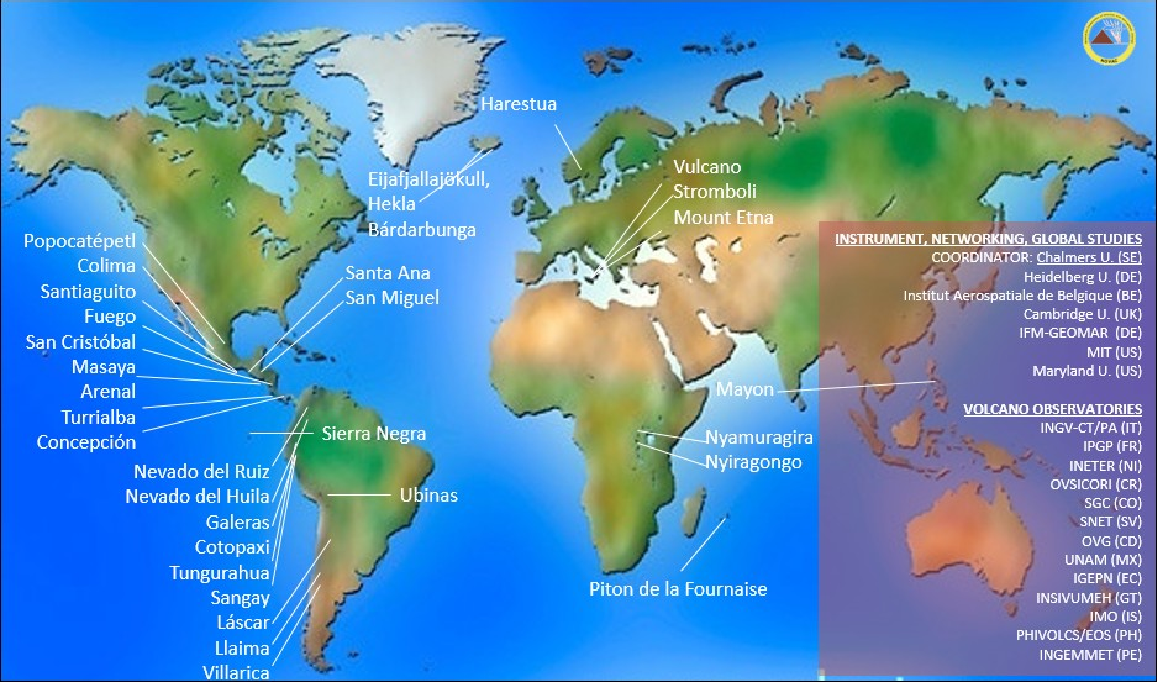
\includegraphics[width=0.8\linewidth]{Bilder/NOVAC2015}
			\caption{Global map of the volcanoes monitored by NOVAC. Used with friendly permission of Santiago Arellano.}
			\label{fig:novac2015}
		\end{figure}
		Network for Observation of Volcanic and Atmospheric Change (NOVAC) is a network of instruments monitoring volcanoes over the hole world. 
		The aim of NOVAC is to gain another tool for risk assessment, for gas emissions and geophysical researches. Also many other scientific purposes are build on the data from NOVAC.\\
		\Cref{fig:novac2015} shows a map, with all volcanoes of the Network for Obersavation of Volcanic and Atmospheric Change.\\
		%
		NOVAC was originally funded by the European Union on the first October in 2005. The aim of NOVAC is to  establish  a  global  
		network  of  stations  for  the  quantitative  measurement  of  volcanic gas  emissions. At the beginning NOVAC encompassed observatories of 15 volcanoes in Africa America and Europe, including some of the most active and strongest degassing volcanoes in the world. Although the EU-funding has stopped, the network has been constantly growing since it was founded. In 2017 more than 80 Instruments are installed at over 30 volcanoes in more than 13 countries.\\
		The great advantage of the data monitored in NOVAC is the fact
		that NOVAC provides continues gas emission data over many years. Therefore one is able to get more statistical stable results.\\
		The instruments used in NOVAC are scanning UV-spectrometer : Mini Doas instruments. \\
		The  Mini-DOAS  instrument  represents  a  major  breakthrough  in  volcanic  gas	monitoring as it is capable of real-time semi-continuous unattended measurement of the total emission fluxes of  SO2	and BrO from a volcano. Semi-continues means in this case that the measurement is only possible during day time when enough Sun light is there.\\
		%
		The  basic  mini-DOAS  system  consists  of  a  pointing  telescope  fiber-coupled  to  a  spectrograph.  
		Ultraviolet light from the sun, scattered from aerosols and molecules in the atmosphere, is collected by 
		means  of  a  telescope  with  a  quartz  lens  defining  a  field-of-view  of  12  mrad.
		\ref{NOVAC Seite} \\
		The spectrometers measure in the UV region in a wavelength range of 280 to 420 nm. In this range are the differential structures of SO2 and BrO dominant.
		\\
 		The Novac-instruments need to be very robust to stand the conditions around volcanoes. Therefore the design of the instruments is rather simple, this means the instruments do not have internal stabilisation features like temperature stabilization to keep the measurement independent of external parameters (for example Temperature).
		This comes along with a reduced precision of the data, but the huge amount of data produced by NOVAC compensates this disadvantage.  
	
	
	\chapter{Measurement Routine}
	The Instruments are set up five to ten km downwind of the volcano of the volcano. To cover most of the occurring wind directions two to five instruments are installed at each volcano. Ideally the measurement plane is orthogonal to the plume, to get the best measurement results. In reality the measurement plane could be twisted.\\
	The Instruments record spectra in different viewing angles covering a the hole sky from horizon to horizon from 
	-90$^{\circ}$ to 90$^{\circ}$. The zenith is at 0$^{\circ}$.
	The measurement routine starts with a spectrum in zenith direction: The pre-reference.
	Afterwards the dark current spectrum is recorded.\\
	Then the Instrument turns automatically to the side, recording spectra at the Elevation Angle from -90$^{\circ}$ to 90$^{\circ}$ with steps of 3.6$^{\circ}$. \\
	One hole measurement takes from 6 to 15 minutes.
	\chapter{Evaluation Routine}
	\section{NOVAC-Evaluation}
	In the following we describe the technical implementation of the DOAS approach using the data of NOVAC instruments:\\
	The first important task is to locate volcano plume and the reference region using the data from te measurement routine described above.
	
	To do so we use the pre-reference (the spectra recorded at an elevation angle of  0$^{\circ} $) to evaluate spectra for SO2 at every elevation angle as described in chapter \ref{DOAS}, that means we divide each recorded spectra by the pre-reference and take the logarithm  to get rid of the Frauenhofer structures and to be able to just look at the important structures of the plume. To get the gas amounts of the evaluated spectra, one fits the absorption spectrum of all important gases on the spectrum. In our case we take all gases written in tab. \ref{tab: 1} into account. The result will be an SO2 curve as it is shown in fig. \ref{fig so2}.
	Figure \ref{fig so2} shows the relative SO2 column density to the pre-reference as a function of the elevation angle. We can clearly observe a a maximum of SO2 and a minimum. Inside the plume the SO2 amount is much higher than in the outside the plume. Therefore we assume that the location of the SO2 maximum match with the location of the plume. We assume that the minimum of the SO2 curve refers to a region outside of the plume which is in most times the case. The SO2 amount in the earths atmosphere is negligible so we take it as a region of zero SO2. Now it is possible to locate the plume region as the SO2 maximum, whereas the minimum of the SO2 curve the reference region is. \\
	To technically detect the plume region we use a gauss fit of the So2 curve.
	To increase the quality and to get a more robust result the sum over several plume spectra is taken. If the gauss curve is too wide we use only the 10 spectra with the highest SO2 amount. For the reference we use the sum of 10 spectra with the lowest SO2 amount.\\
	%
	The so found reference spectrum is used to fit it on the SO2 absorption lines of Gases to get the absolute column densities of SO2 and BrO in the plume spectrum\\
	\\
	Since the BrO column density is much lower than the SO2 column density and lies just slightly above the detection limit the plume is hard to detect using the BrO column density as it is shown in fig. \ref{ fig bro}. 
	Therefore we use plume location we found by using SO2 to evaluate the BrO column density.\\
	For the evaluation we use the data of more than one measurement, to increase the fit quality.\\
	We are mainly interested in the BrO/SO2 ratio, with the calculations described above it is now possible the get this ratio.
	In \cref{...} is the NOVAC Evaluation visualized.
	
	

	\section{Contamination Problem}
	\begin{figure}
		\centering
		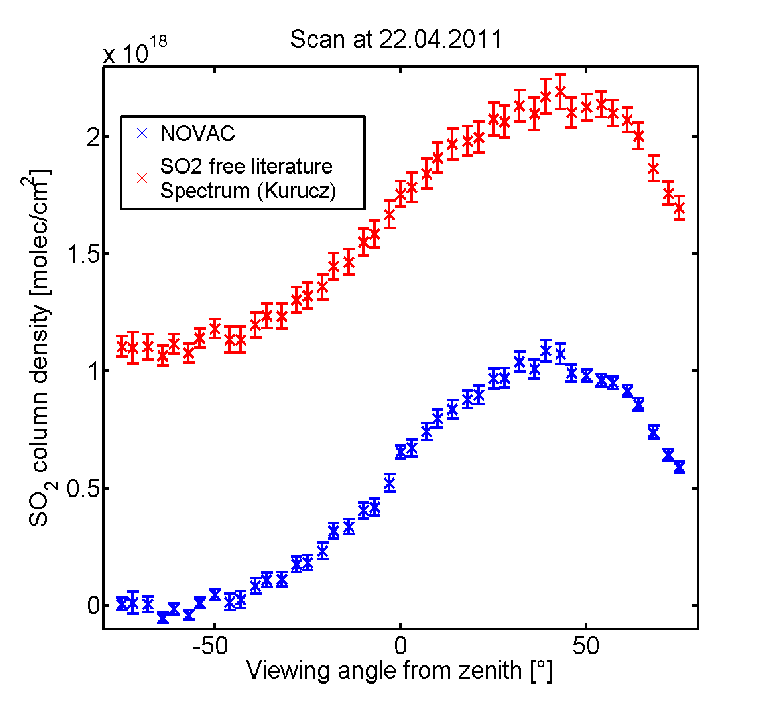
\includegraphics[width=0.7\linewidth]{Bilder/contaminated}
		\caption{}
		\label{fig:contaminated}
	\end{figure}
	
	It might occur that in rare (ca. 10\% of the data) scenarios, the
	volcanic plume covers the whole scan region.
	This could happen if for example the volcanic plume of the day before still extend over the hole scan area as a consequence of windless conditions.
	In consequence, the reference	is contaminated with volcanic trace gases. Thus the gas amount is underestimated by the NOVAC-Evaluation: In \cref{fig:contaminated} we see an example from April 2011 (Tungurahua) where the reference region is contaminated by volcanic trace gases. The blue SO2 curve shows our calculations with the NOVAC-Evaluation, but since there is still SO2 in the reference region, therefore the assumption, that the SO2 amount could be set to zero in the reference region is wrong. The red curve shows the real SO2 curve, and we will underestimate the total SO2 amount of the plume. Contamination occur in approximately 10$\%$ of the data.\\
	\\
	If the reference region is for any reason
	contaminated by volcanic trace gases, the reference spectrum has to be
	replaced by a volcanic-gas-free reference. Alternative spectra are a
	theoretical solar atlas spectrum (the use of a solar atlas spectrum will be described in \cref{kuruz}) ore a a volcanic-gas-free reference
	spectrum recorded by the same instrument.\\ 
	%
	\\
	%
	In the following we will discuss both of these options:
	%
	\subsection*{Evaluation using a Solar Atlas Spectrum \label{kuruz}}
	An alternative to choose the region with the lowest column density as reference region is to use a theoretical high resolution solar atlas spectrum as reference \cite{chance2010improved}.
	The use of a theoretical solar atlas spectrum as a reference which is completely volcanic-trace-gases-free was first proposed by \cite{lubcke2014bro}.
	The advantage of using a solar atlas spectrum as reference is, that we know that there are no volcanic trace gases, we do not need to assume, that the minimum SO2 amount is zero. The disadvantage is, that using a solar atlas spectrum comes along with a drawback of precision: A theoretical solar atlas spectrum is far more precise than the spectra of the NOVAC instruments therefore the instrument functions need to be modeled and added to the retrieval.\\ 
	The reduction of precision is acceptable for the
	SO2 retrieval but not suitable for a BrO retrieval because then most data would be below the detection limit.\\
%
\\
%
	Possible contaminations can be checked
	by a theoretical solar atlas spectrum to evaluate the SO2 amount in the reference.

	\subsection*{Evaluation using a Spectrum of the same Instrument}
	An alternative reference spectrum coud be a a volcanic-gas-free reference
	spectrum recorded by the same instrument. When using such a reference several problems occur:\\
	As described in \cref{NOVAC} the instruments used in NOVAC do not include features like temperature stabilisation due to that the measurements are not independent from external parameters. 
	So we need to choose a reference recorded at similar conditions with respect to meteorology and	radiation as well as in the temporal proximity due to instrumental changes with time and ambient conditions. Ideally the external conditions should be equal to the conditions when the plume was recorded.\\
	\\
	%
	\\
	In this work we will combine both options in order to
	achieve both, enhanced accuracy but still maximum possible precision of
	the SO2 and BrO retrievals. So we use the solar atlas spectrum to check for 
	contamination and a reference spectrum recorded in temporal proximity by the same instrument as reference.\\
	\\
	%
	\\
	In the following we will discuss how to find the an optimal reference from another scan automatically.
	
	\begin{figure}
		\centering
		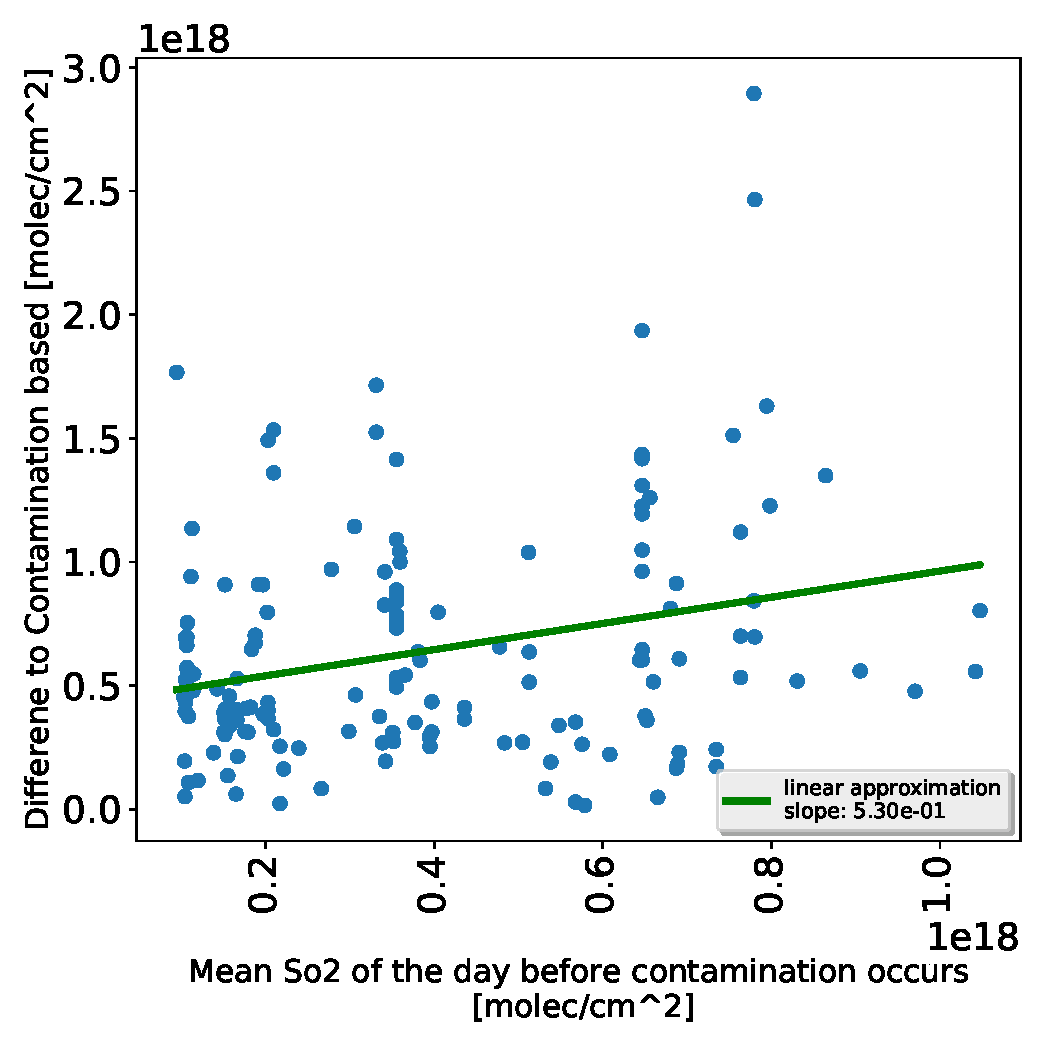
\includegraphics[width=0.7\linewidth]{E:/Masterarbeit/Analyse_Contamination/contaminationdependency_so2}
		\caption{}
		\label{fig:contaminationdependencyso2}
	\end{figure}
	\begin{figure}
		\centering
		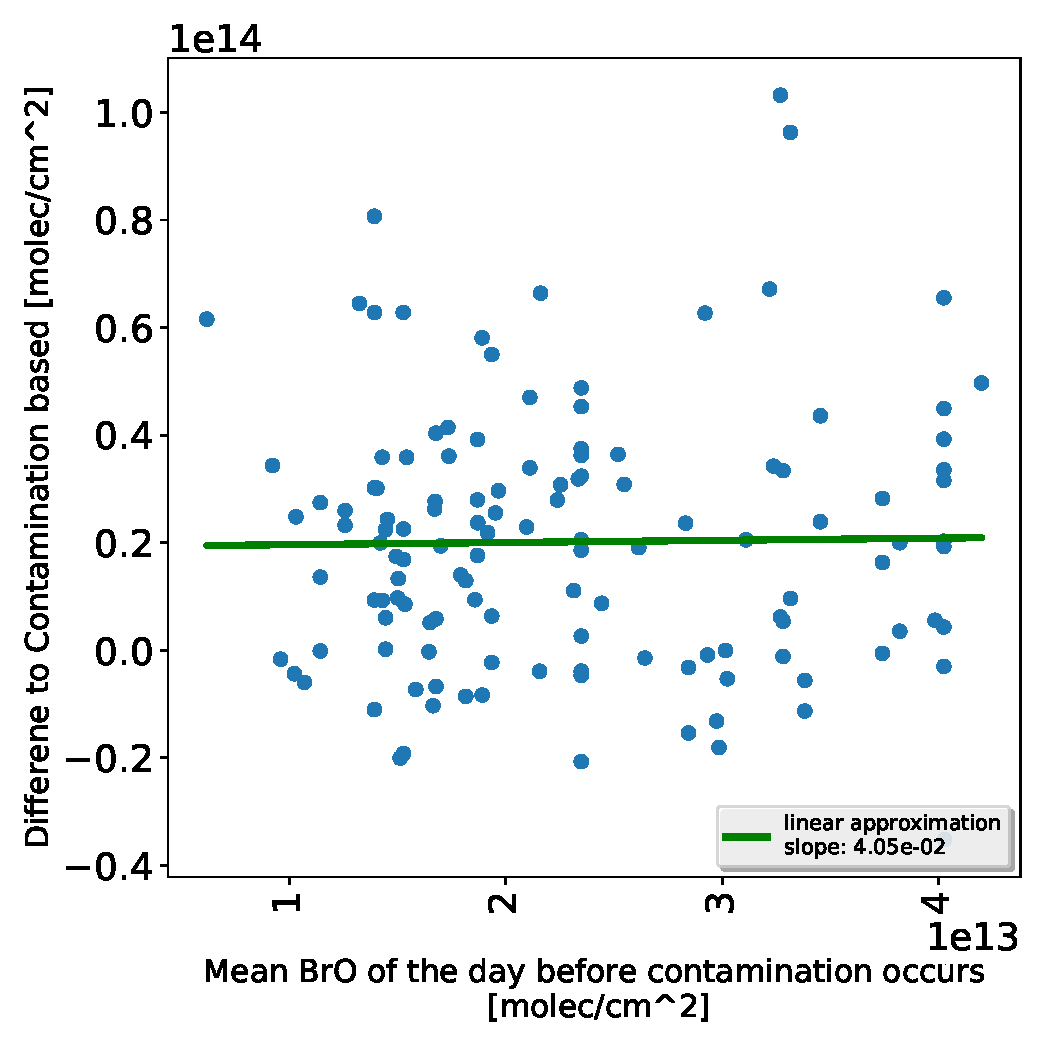
\includegraphics[width=0.7\linewidth]{E:/Masterarbeit/Analyse_Contamination/contaminationdependency_bro}
		\caption{}
		\label{fig:contaminationdependencybro}
	\end{figure}
	\begin{figure}
		\centering
		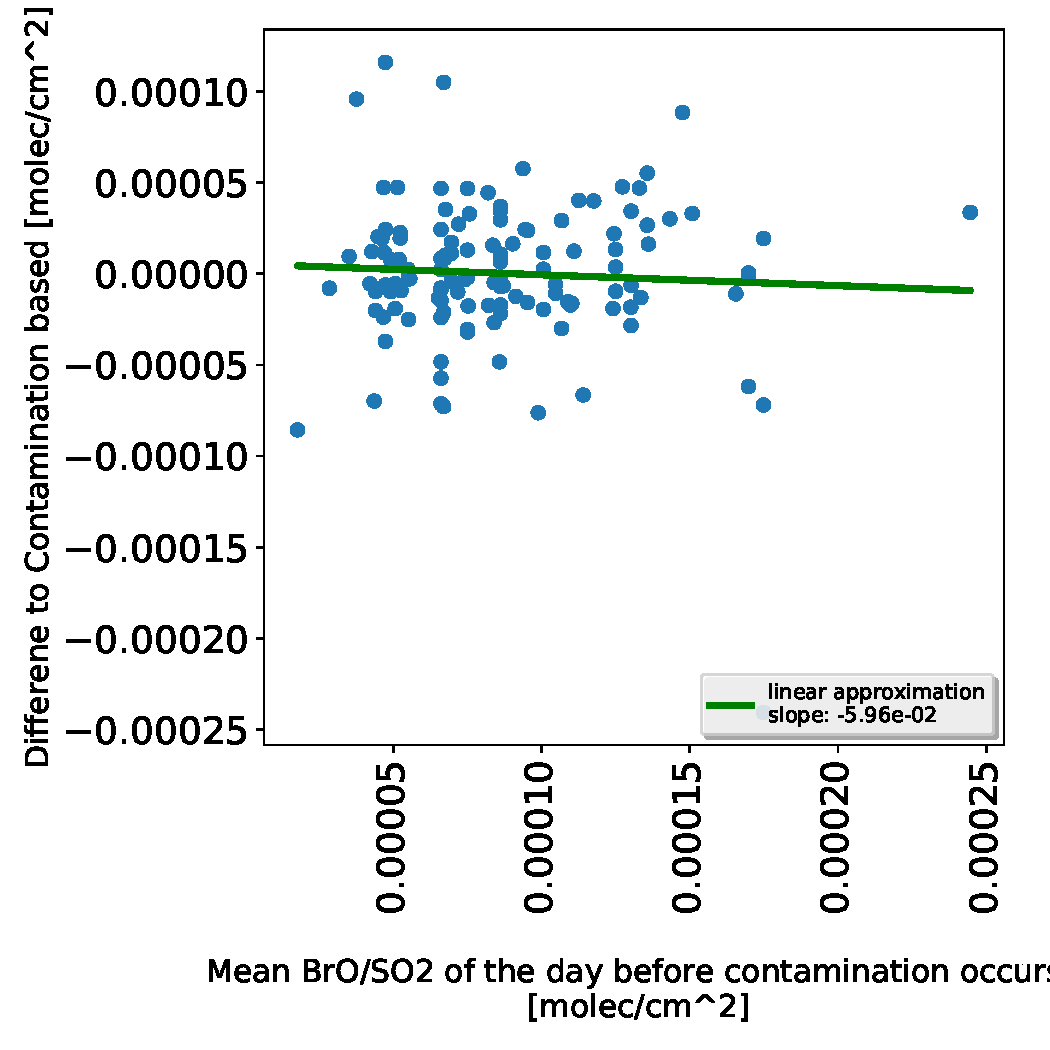
\includegraphics[width=0.7\linewidth]{E:/Masterarbeit/Analyse_Contamination/contaminationdependency_ratio}
		\caption{}
		\label{fig:contaminationdependencyratio}
	\end{figure}
	\chapter{Limitations for the evaluation of  BrO}
    Since the SO2 amount in a volcano plume is rather high (magnitude of SO2 at Tungurahua $\approx 1e^{18}$, \cite{WarnachSimon}) , the evaluation of SO2 is unproblematic compared to BrO.\\
	Evaluating BrO is more difficult since the amount is much smaller and the measurement error relative to the column density much larger. Since we want to get the BrO/SO2 we need to maximize the accuracy of BrO.
	Therefore the aim is to choose the reference with respect to the BrO error, to minimize the BrO Error and to increase the amount of reliable BrO/SO2 ratio data.\\
	We figured out, that the BrO Error depends strongly on the surrounding conditions when recording the plume and the reference. In the following, we will take a closer look at the dependence of the BrO error on external parameters. 
	%
	\section{BrO Error dependence on external parameters}
	%HOW IS THE ERROR CALCULATED AND WHY AND DETECTION LIMIT (PLATT \& STUTZ)
	The measurement and evaluation depends on the surrounding conditions like temperature or cloudiness \cite{lubcke2014optical}\\
	If choosing a new reference we need to take the surrounding conditions into account\\
	The better the surrounding conditions of the time where the reference is measured coincide with the conditions of the time when the plume is measured, the lower is the BrO error \\
	The surrounding conditions we take into account are temperature, colorindex, exposure time, elevation-angle, daytime and the temporal difference.\\
	In almost all cases (99\%) the absolute BrO Error is minimal when using the reference recorded at the same time as te plume spectrum. So we won't be able to get an BrO Error which is smaller than the "Same Time Error".   

	
	\subsection{Time}
	Due to instrument drifts the fit quality decreases with the time difference between recording the plume and the reference. Therefore it is better to use an reference in temporal proximity.\\
	%
	\Cref{shiftPic} shows the Instrumental drift as a function of time, to create \cref{shiftPic} we used Tungurahua data, 2008 from June to November. We can observe that the drift changes with time. If we use the reference and plume spectra of the same time, we do not need to care about these effects, since the shift is equal for the plume and reference spectrum, but if the recording time is not the same the quality of the fit changes with the differences in wavelength shift which increases with the time difference.\\
	In \cref{fig:dat} the BrO Error as a function of the time difference between recording the plume and the reference is shown. The running mean is drawn with a black line. The BrO Error increases with time difference.\\
	To evaluate the maximal time difference, were we still get reliable results we calculated for all possible reference-plume pairs the corresponding BrO Error. With this data we are able to find for all plume spectra the associated reference where the BrO Error is minimal. In \cref{Histogram} a histogram is plotted with the probability of picking the best reference as a function of the time difference. Obviously the best results are if the day of measuring the reference is the same day as measuring the reference that means, if the time difference is smaller than one day. We allow all time difference which are in one sigma area. 
	
	We found out that the time interval where it is still reasonable to use references is about 14 days. Therefore we only use references where the recording time difference between plume and reference is smaller than two weeks. When using a references with a temporal difference to the plume of more than 14 days the probability, that the fit quality and thus the BrO error increases to much for our purposes. \\
	\\

	\begin{figure}
		\centering
		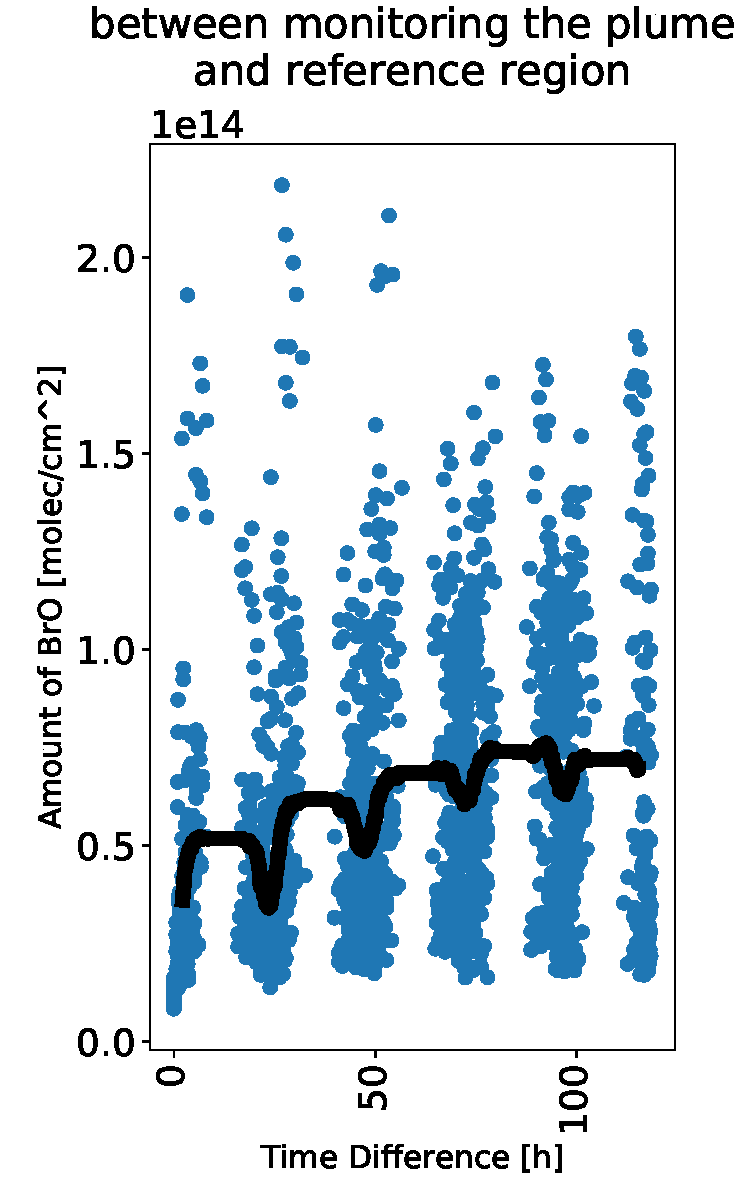
\includegraphics[width=0.7\linewidth]{Bilder/Datum_100h}
		\caption{}
		\label{fig:datum100h}
	\end{figure}
	
	\begin{figure}[h!]
		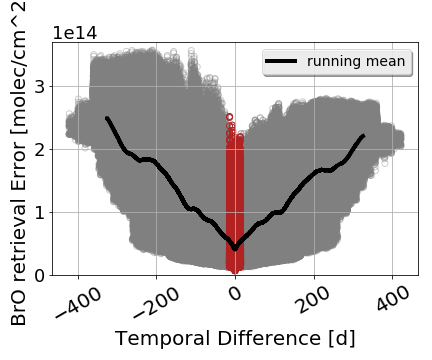
\includegraphics[width=1.1\linewidth]{Bilder/Datum}
		\caption{}
		\label{fig:dat}
	\end{figure}

	\subsection{Temperature}
	%einbinden einer Grafik
	\begin{figure}[h!]			
		\subfigure[Data of Tungurahua]{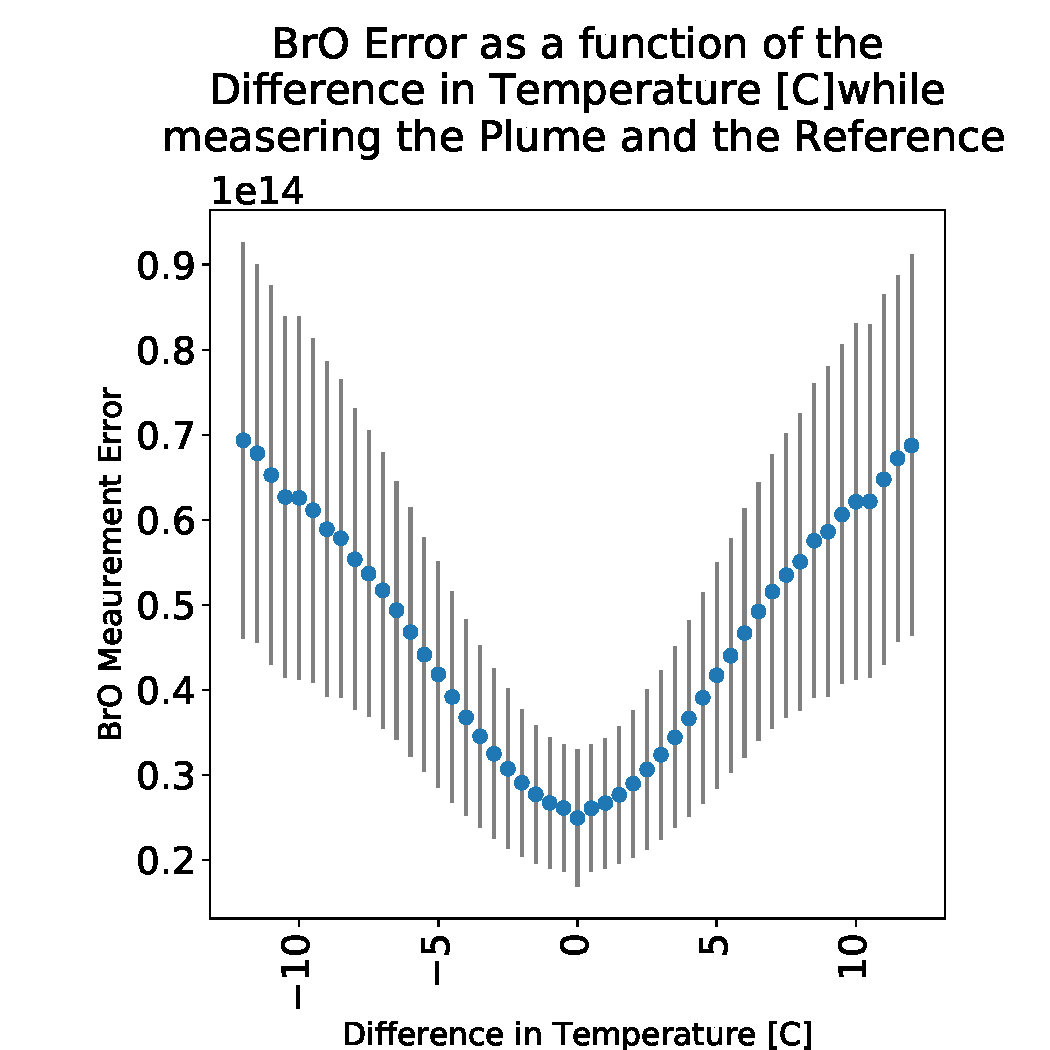
\includegraphics[width=0.49\textwidth]{Bilder/DiffTemp_Tungu}}
		\subfigure[Data of Nevado Del Riz]{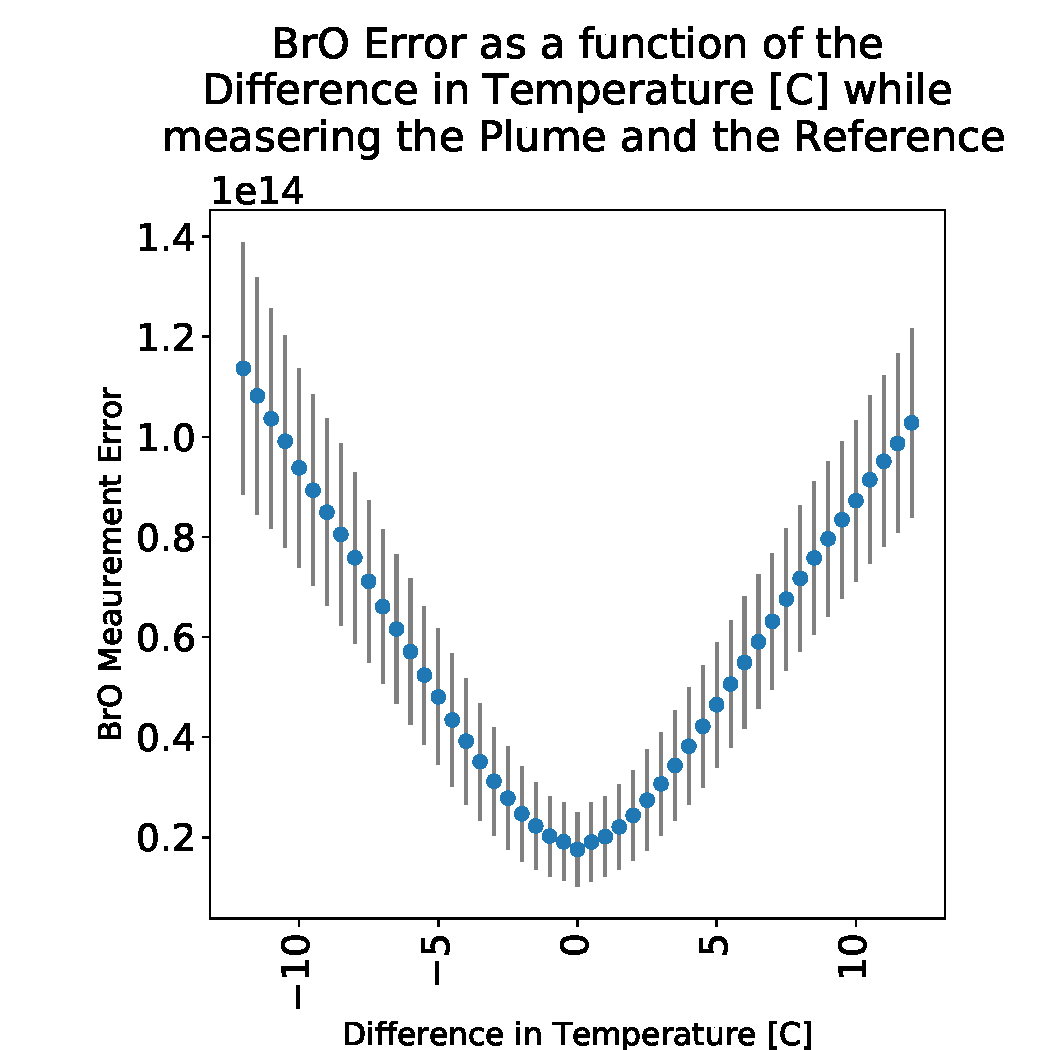
\includegraphics[width=0.49\textwidth]{Bilder/DiffTemp_Nevad}}
		\caption{Titel unterm gesamten Bild}
	\end{figure}
	\begin{itemize}
		\item The BrO error has the strongest dependence on the temperature difference. At Tungurahua (Nevado Del Ruiz) the BrO error increases by factor of $3.53\cdot10^{12}$  per degree.
		\begin{align*}
		\rightarrow&  BrO_{Error} = f(ext. P)+ 3.53\cdot10^{12}\cdot\frac{\Delta T}{1C^{\circ}} + \mathcal{O}\left(\right) & Tungurahua\\
		\rightarrow&  BrO_{Error} = f(ext. P)+7.56\cdot10^{12}\cdot\frac{\Delta T}{1C^{\circ}} + \mathcal{O}\left(\right) & Nevado Del Ruiz\\
		\end{align*}
	\end{itemize}
	\subsection{Daytime}
	\begin{figure}[h!]			
		\subfigure[Data of Tungurahua]{\includegraphics[width=0.49\textwidth]{Bilder/Diffdaytime_Tungu}}
		\subfigure[Data of Nevado Del Riz]{\includegraphics[width=0.49\textwidth]{Bilder/Diffdaytime_Nevad}}
		\caption{Titel unterm gesamten Bild}
	\end{figure}
	\begin{itemize}
		\item We found a dependency of the BrO error on the daytime. We assume, that this dependency comes from other external parameters which change during the day. 
		\item The BrO Error increases with the daytime differences like: \\
		\begin{align*}
		\rightarrow&  BrO_{Error} = f(ext. P)+1.33\cdot10^{12}\cdot\frac{\Delta DT}{1h}  + \mathcal{O}\left(\right)& Tungurahua\\
		\rightarrow&  BrO_{Error} = f(ext. P)+1.58\cdot10^{13}\cdot\frac{\Delta DT}{1h} + \mathcal{O}\left(\right) & Nevado Del Ruiz\\
		\end{align*}
		
	\end{itemize}
	\subsection{Colorindex}
	\begin{figure}[h!]		
		\subfigure[Data of Tungurahua]{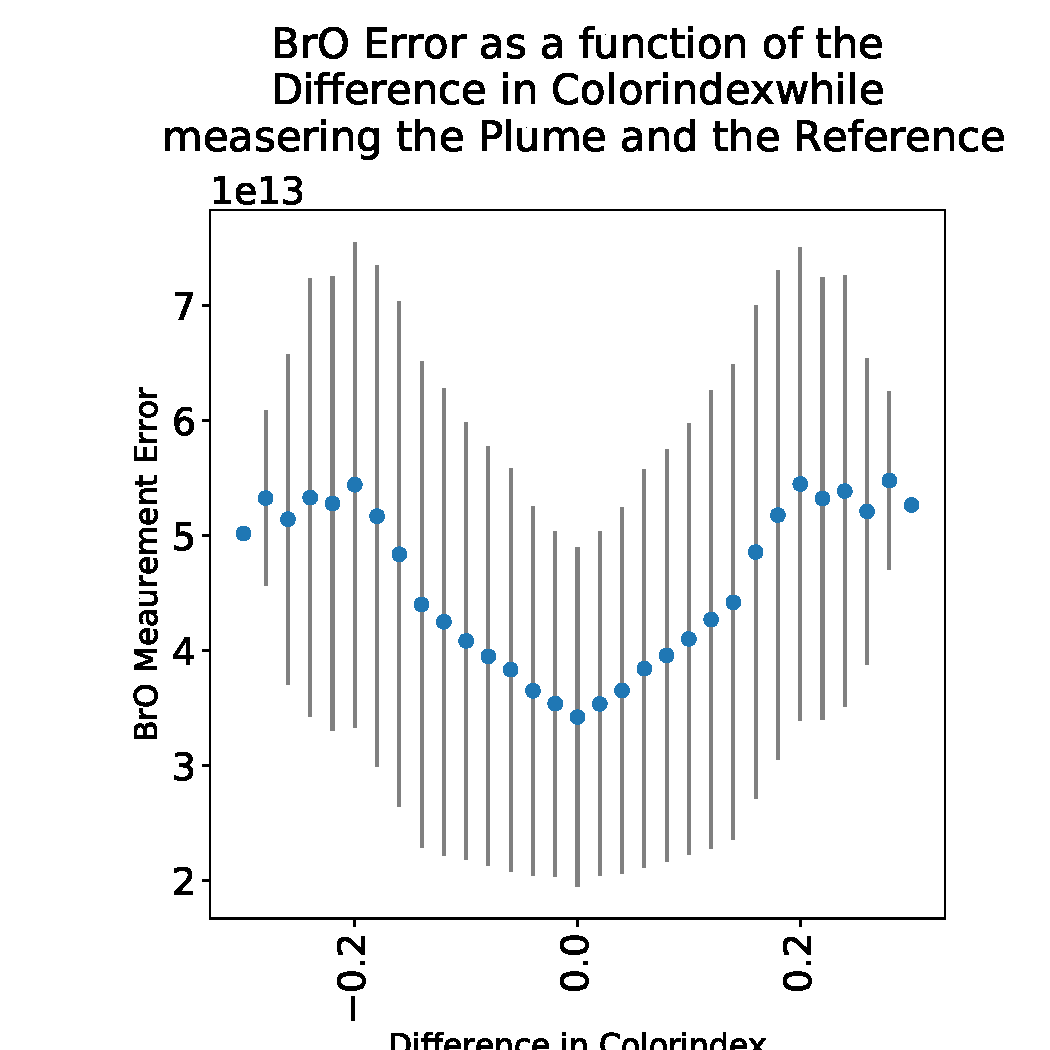
\includegraphics[width=0.49\textwidth]{Bilder/DiffColidx_Tungu}}
		\subfigure[Data of Nevado Del Riz]{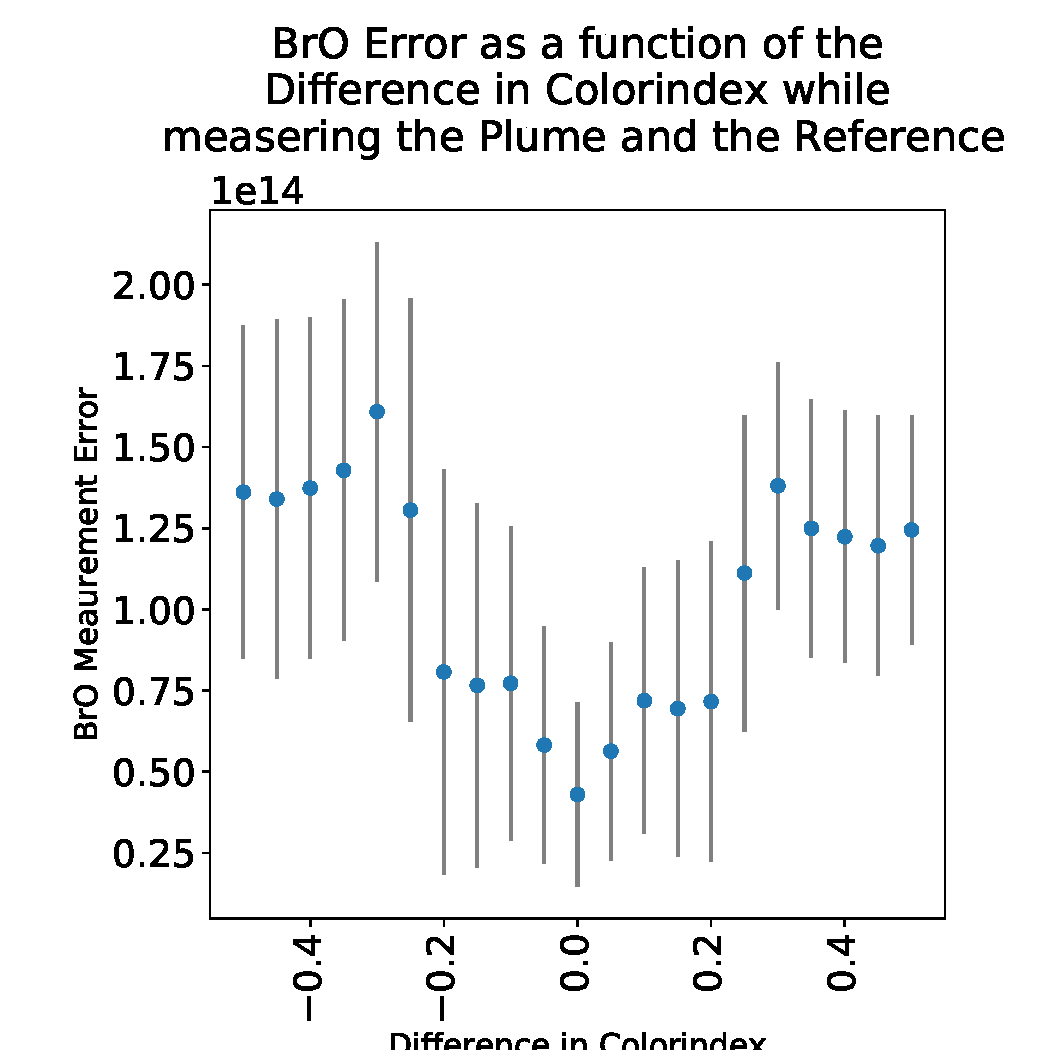
\includegraphics[width=0.49\textwidth]{Bilder/DiffColidx_Nevad}}
		\caption{Titel unterm gesamten Bild}
	\end{figure}
	\begin{itemize}
		\item 	The BrO Error increases with the Colorindex differences as \\
		\begin{align*}
		\rightarrow&  BrO_{Error} = f(ext. P)+ 1.01\cdot10^{13}\cdot\frac{\Delta Cidx}{0.1} + \mathcal{O}\left(\right) & Tungurahua\\
		\rightarrow&  BrO_{Error} = f(ext. P)+  4\cdot10^{13}\cdot\frac{\Delta Cidx}{0.1} + \mathcal{O}\left(\right) & Nevado Del Ruiz\\
		\end{align*}
	\end{itemize}
	\subsection{Elevation Angle}
	\begin{figure}[h!]			
		\subfigure[Data of Tungurahua]{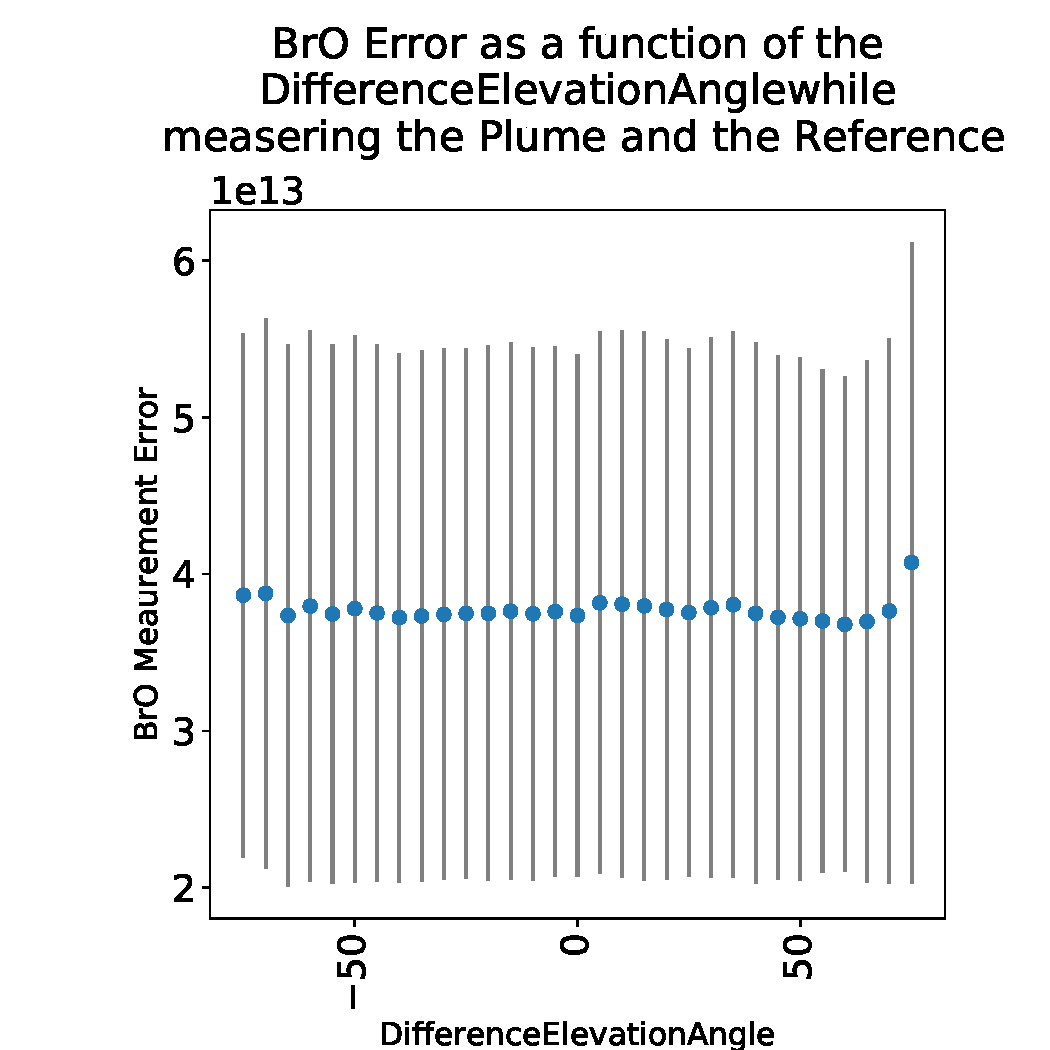
\includegraphics[width=0.49\textwidth]{Bilder/DiffElevAngle_Tungu}}
		\subfigure[Data of Nevado Del Riz]{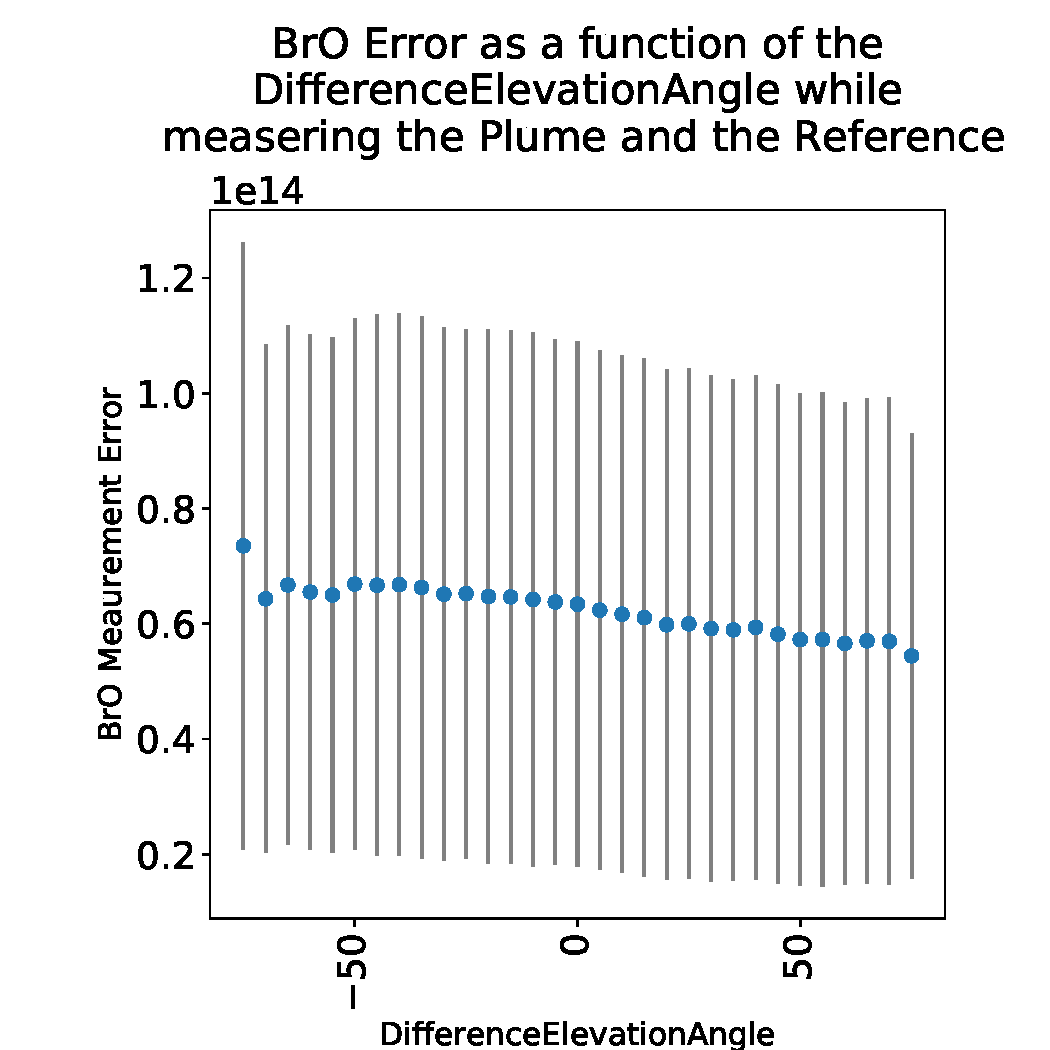
\includegraphics[width=0.49\textwidth]{Bilder/DiffElevAngle_Nevad}}
		\caption{Titel unterm gesamten Bild}
	\end{figure}
	\begin{itemize}
		\item 	The BrO error doesn't depend significantly on the difference between the Elevation Angles. This could have several reasons. One problem is, that the Elevation Angle of Plume and Reference spectrum is not the same. This could also be a reason of uncertainty of the evaluations of the plume spectrum.
	\end{itemize}
\begin{figure}
	\centering
	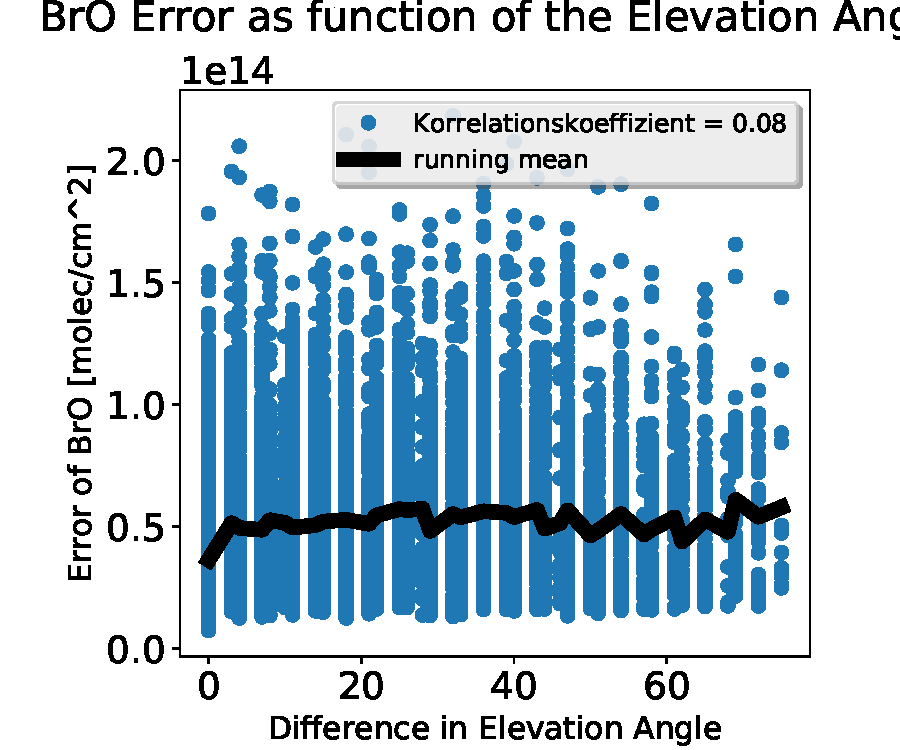
\includegraphics[width=0.7\linewidth]{Bilder/AbsofElevationAngleAsFunctionofBrOError_AllData}
	\caption{}
	\label{fig:absofelevationangleasfunctionofbroerroralldata}
\end{figure}

	\subsection{Exposure Time}
	\begin{figure}		
		\subfigure[Data of Tungurahua]{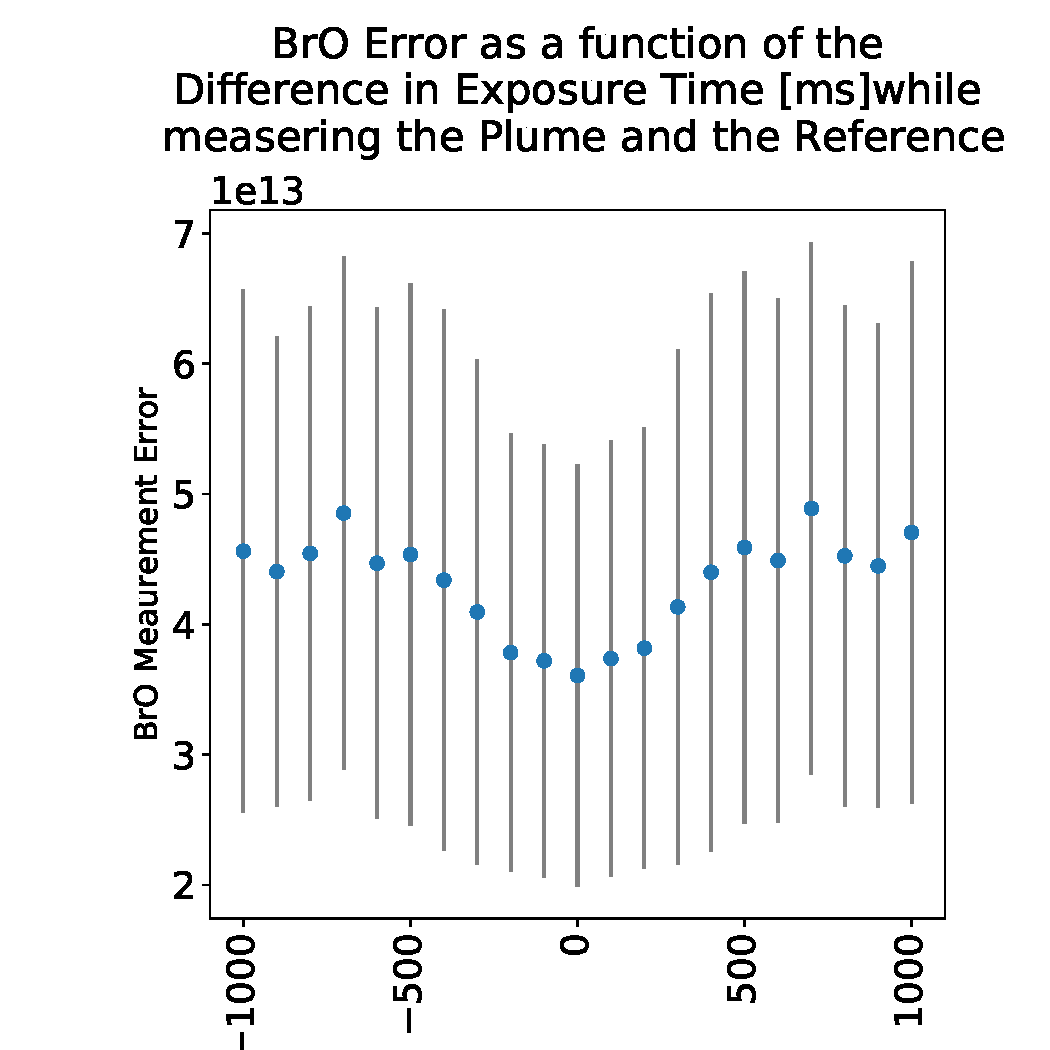
\includegraphics[width=0.49\textwidth]{Bilder/DiffExpTime_Tungu}}
		\subfigure[Data of Nevado Del Riz]{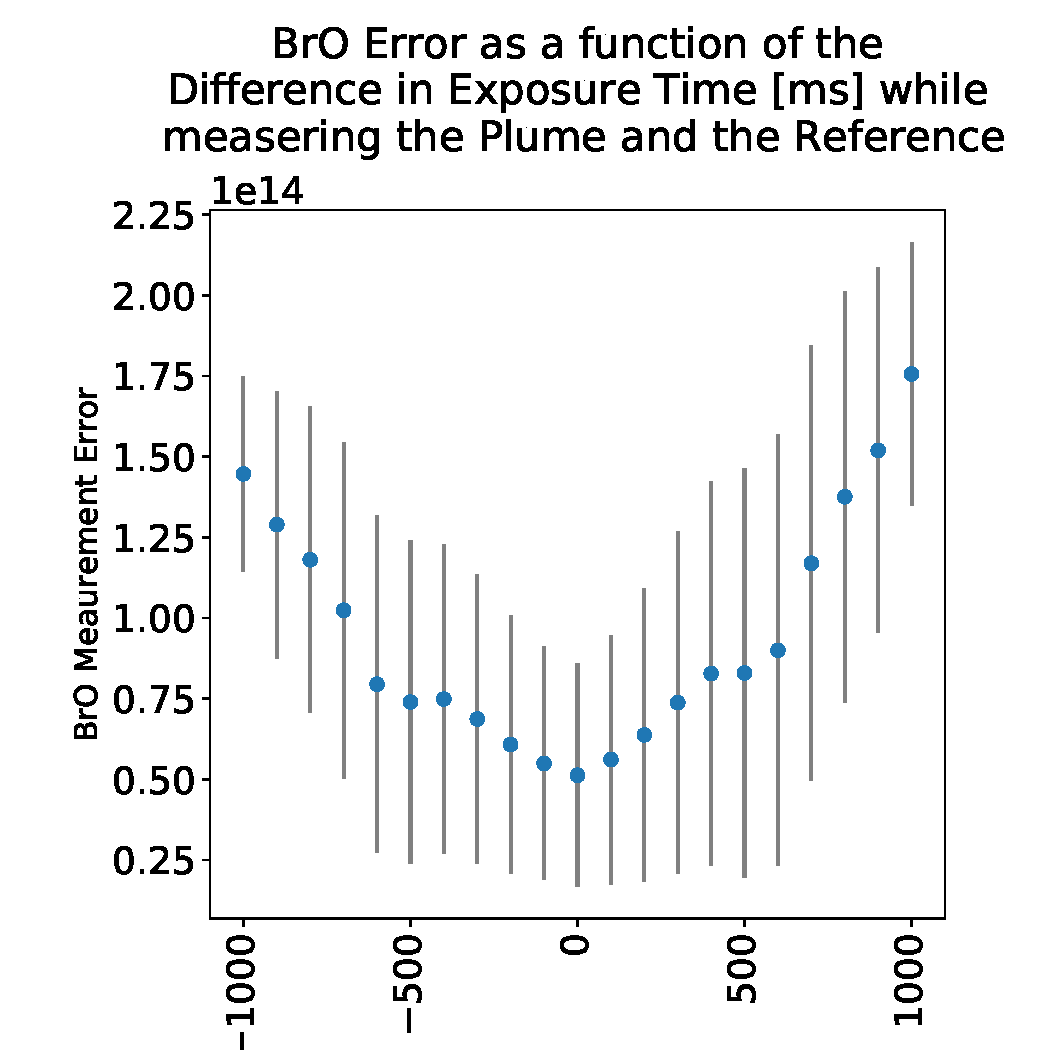
\includegraphics[width=0.49\textwidth]{Bilder/DiffExpTime_Nevad}}
		\caption{Titel unterm gesamten Bild}
	\end{figure}
	\begin{itemize}
		\item The BrO Error increases with the exposure time differences as\\
		\begin{align*}
		\rightarrow&  BrO_{Error} = f(ext. P)+ 1.92\cdot10^{12}\cdot\frac{\Delta ET}{10^{-2}s} + \mathcal{O}\left(\right) & Tungurahua\\
		\rightarrow&  BrO_{Error} = f(ext. P)+ 1.0\cdot10^{13}\cdot\frac{\Delta T}{10^{-2}s} + \mathcal{O}\left(\right) & Nevado Del Ruiz\\
		\end{align*}
	\end{itemize}
	%--------------------------------------------------------------------------------------------------------------
	\chapter{Method}
	\section{Fit data}
	\begin{itemize}
		\item A Spectrum is treated as contaminated if the SO2 column density of the reference (evaluated with a solar atlas spectrum) is larger as 2$\cdot 10^{17}\frac{molec}{cm^2}$.
		\item Plume data are reliable if the SO2 column density is larger as 7 $\cdot 10^{17} \frac{molec}{cm^2}$
		\item Data are above the detection limit if the column density as two times larger than the fit error.
		\item If the reference is contaminated:
		\begin{itemize}
			\item We have a list of possible references where all references are not contaminated and the temporal distance to the plume date is no longer than 14 days.
			\item we calculate of all possible references the differences in the external parameters
			\item We use the analyse of external parameters described above to estimate the BrO error of all references
			\item We choose the reference with the smallest estimated BrO error as new reference
			\item We evaluate the plume spectra with the new reference.
		\end{itemize}
	\end{itemize}
\begin{figure}
	\centering
	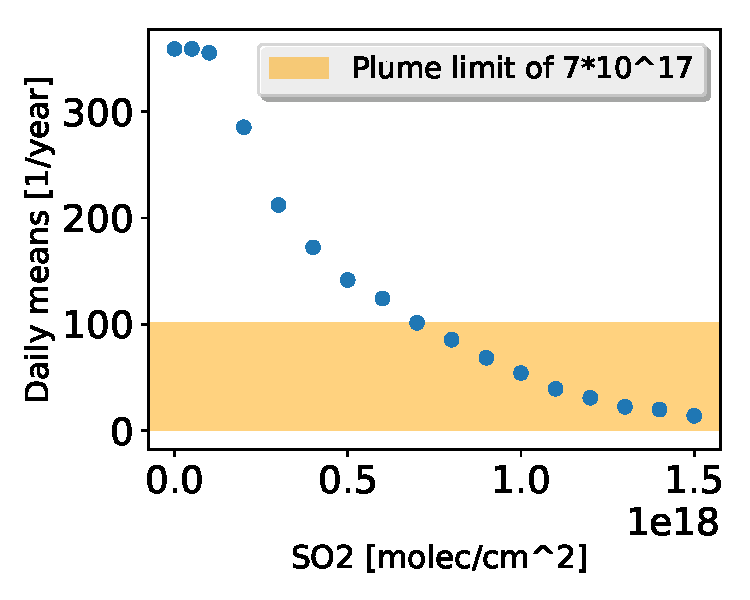
\includegraphics[width=0.7\linewidth]{E:/Masterarbeit/Analyse_minSO2/percentage_minSO2}
	\caption{}
	\label{fig:percentageminso2}
\end{figure}
\begin{figure}
	\centering
	\includegraphics[width=0.7\linewidth]{E:/Masterarbeit/Analyse_minSO2/data_minSO2}
	\caption{}
	\label{fig:dataminso2}
\end{figure}

	\section{Other approaches}
	\begin{itemize}
		\item We also tried other possibilities than fitting to find the reference where the BrO error is minimal. In the following we present two additional possibilities but compared to fitting the results are not as good.
	\end{itemize}
	\subsection{Nearest neighbours}
	\begin{itemize}
		\item Description of the Nearest Neighbours Method
	\end{itemize}
	\subsection{Iterative}
	\begin{itemize}
		\item Description of the iterative Method
	\end{itemize}
	\chapter{Comparison with NOVAC Evaluation}
	\begin{itemize}
		\item Results only for contaminated data
		\begin{itemize}
			\item Difference in SO2 data evaluated with NOVAC-method and contamination-based evaluation
			\item Difference in BrO data evaluated with NOVAC-method and contamination-based evaluation
			\item Difference in BrO/So2 Ratio data evaluated with NOVAC-method and contamination-based evaluation
		\end{itemize}
		\item More BrO data: 51\%
		\item  More valid BrO data: 38\%
	\end{itemize}
	\chapter{Results}
	Interpretation of the BrO/SO2 ratio time-series
	\section{Tungurahua}
	\begin{small}	
	\begin{align*}
	&Menge an Daten insgesamt: &5883 &\equiv &1\\
	&\hspace*{1cm} Davon: (NOVAC Auswertung) über plume limit&712 &\equiv & 0.121\\
	&\hspace*{1cm}Davon: Menge an Daten, die nicht Kontaminiert sind: &5504 &\equiv & 0.936\\
	&\hspace*{2cm}Davon im Plume-limit:  &599   &\equiv & 0.102\\
	&\hspace*{2cm}Davon über dem Detection Limit:&36  &\equiv & 0.006\\
	&\hspace*{1cm}Davon sind kontaminiert:  &379  &\equiv & 0.064\\
	&\hspace*{2cm}Davon (mit NOVac ausgewertet) über plume limit: &114  &\equiv &0.301 \\
	&\hspace*{2cm}Davon (Neue Auswertung) über plume limit &185  &\equiv &0.488\\
	\end{align*}	
	Dh in den kontaminierten daten sind mit NOVAC ausgewerteten daten \underline{2.485} häufiger über dem plume limit\\	

	\end{small}
	\section{Nevado Del Ruiz}
	\begin{small}	
	\begin{align*}
		&Menge an Daten insgesamt:  &8962 &\equiv &1\\
		&\hspace*{1cm} Davon: (NOVAC Auswertung) über plume limit&142  &\equiv &0.016\\
		&\hspace*{1cm} Davon: nicht kontaminierte daten: &8596 &\equiv &0.959\\
		&\hspace*{2cm} Davon im Plume-limit:   &123  &\equiv &0.014\\
		&\hspace*{2cm} Davon über dem Detection Limit: &53   &\equiv &0.006\\
		&\hspace*{1cm} Davon sind kontaminiert:  &366  &\equiv &0.041\\
		&\hspace*{2cm} Davon (mit NOVac ausgewertet) über plume limit: &20   &\equiv &0.055\\
		&\hspace*{2cm} Davon  (Neue Auswertung) über plume limit&179 &\equiv &0.489\\
		\end{align*}
	Dh in den kontaminierten daten sind mit NOVAC ausgewerteten daten \underline{3.449} häufiger über dem plume limit\\
 	
 \end{small}
	\chapter{Issues of our method}
	\section{Contamination of the plume}
	\begin{itemize}
		\item As discussed above it might occur, that, that the reference is contaminated for example by the plume of the day before. If that happens, we underestimate the gas amount by using a contaminated reference. But another possibility is, that the plume is also contaminated. This might be the case if the volcanic gas of the volcano is not taken away by the wind, but accumulates in the plume. If this is the case, using an other reference would lead to an overestimation of the column density of gases.
	\end{itemize}

	\chapter{Conclusion}
	....
	
	
	



  \part{Appendix}
  \begin{appendix}
    \chapter{Lists}
    \listoffigures
    \listoftables
    \bibliography{references}{}
    \citestyle{egu}
    \bibliographystyle{plainnat}
    \setlength{\parindent}{0em}

Erkl\"{a}rung:\par
\vspace{3\baselineskip}
Ich versichere, dass ich diese Arbeit selbstst\"{a}ndig verfasst habe und keine
anderen als die angegebenen Quellen und Hilfsmittel benutzt habe.\par
\vspace{5\baselineskip}
Heidelberg, den (Datum)\hspace{3cm}\dotfill

  \end{appendix}
\end{document}




